\documentclass{beamer}
\usepackage[spanish]{babel}
\usepackage[latin1]{inputenc}
\usetheme{Warsaw}
\useoutertheme{shadow}


\begin{document}

\begin{frame}
    \frametitle{BrainStorm optimization}
    \begin{figure}
		\centering
		
\includegraphics[width=0.7\linewidth]{blog_brainstorming}
		\label{fig:blog_brainstorming}
	\end{figure}

\end{frame}

\begin{frame}
	\frametitle{Brainstorm optimization}
	Se basa en el comportamiento humano para resolver problemas.
	\begin{itemize}
		\item \textbf{Generar primeras ideas sin prejuicios} 
		\item \textbf{Agrupar ideas parecidas}
		\item \textbf{Fusionar ideas prometedoras pero de distintos grupos}
		\item \textbf{Intentar mejorar buenas ideas.}
	\end{itemize}
\end{frame}

\begin{frame}
	\frametitle{Brainstorm optimization}
	\textbf{Generaci�n de ideas}
	
	\begin{figure}
		\centering
		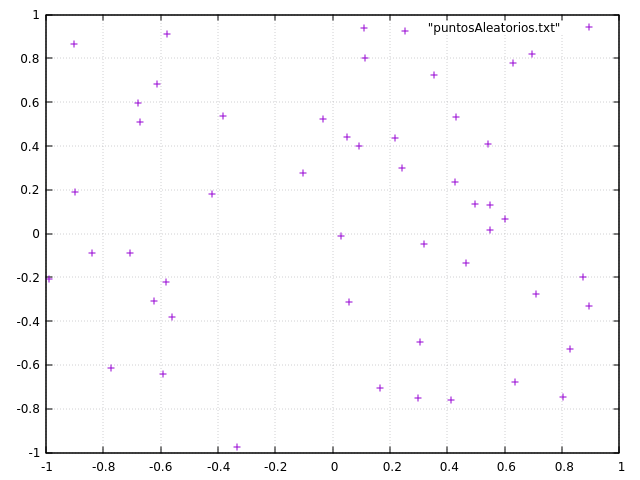
\includegraphics[width=0.7\linewidth]{PrimerasIdeas}
		\label{fig:PrimerasIdeas}
	\end{figure}

\end{frame}

\begin{frame}
	\frametitle{Brainstorm optimization}
	\begin{figure}
		\centering
		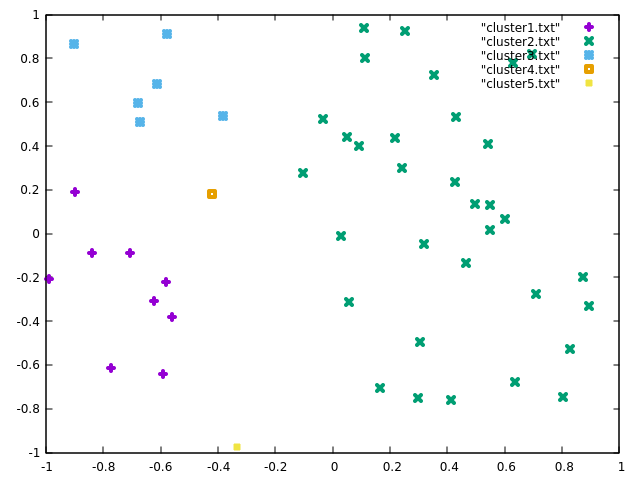
\includegraphics[width=0.7\linewidth]{clusterIdeas}
		\label{fig:clusterIdeas}
	\end{figure}

\end{frame}

\begin{frame}
	\frametitle{Brainstorm optimization}
	
	\[coste(x) = \sum \left| cos(x_i) \right| \]
	\begin{figure}
		\centering
		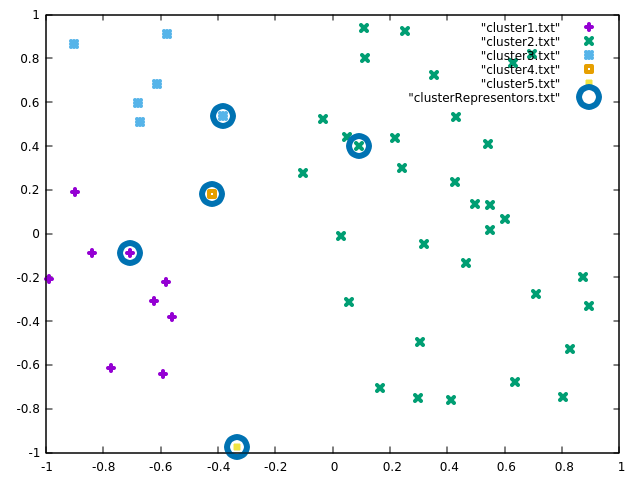
\includegraphics[width=0.7\linewidth]{representantesCluster}
		\label{fig:representantesCluster}
	\end{figure}

	
\end{frame}

\begin{frame}
	\frametitle{Brainstorm optimization}
	\begin{itemize}
		\item \textbf{Posible mutaci�n de alg�n representante de cluster.}
		
		\begin{itemize}
			\item  \[X^d_{new} <-X^d_{selected} + \psi \times n(0,1) \]
		
			\item \[\psi = logsig\left(\dfrac{\dfrac{Max_{iter}}{2}-Curr_{iter}}{k}\right)\times random()\]
		\end{itemize}
		
	\end{itemize}
		
	
\end{frame}

\begin{frame}
	\frametitle{Brainstorm optimization:par�metros de modificaci�n}
	
	\begin{figure}
	\centering
	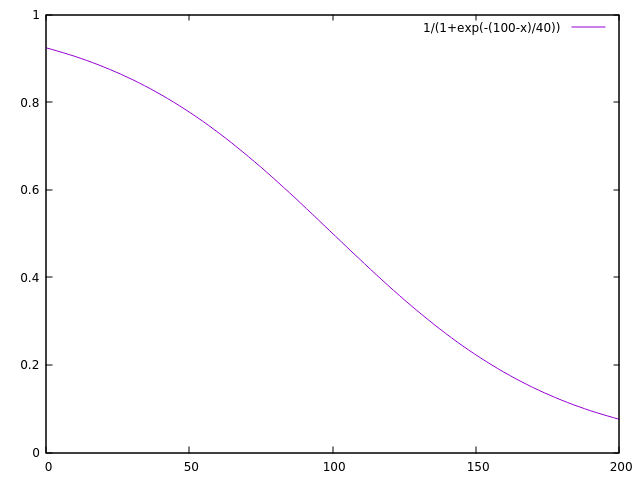
\includegraphics[width=0.4\linewidth]{logsig.png}
	\label{fig:logsig}
	\end{figure}
	
	\begin{figure}
		\centering
		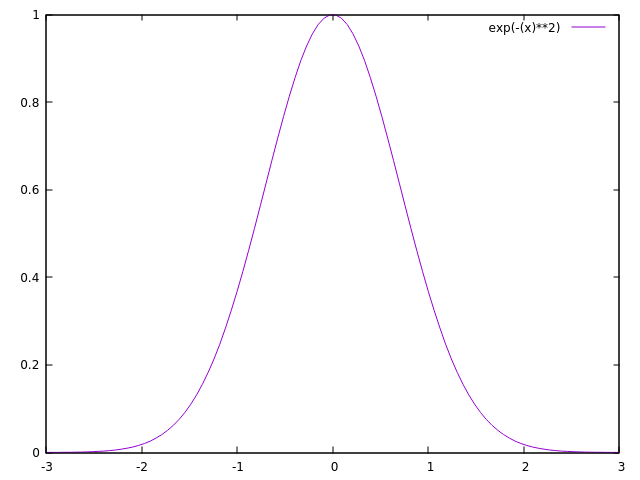
\includegraphics[width=0.4\linewidth]{normal.png}
		\label{fig:normal}
	\end{figure}
	
\end{frame}





\end{document}